\chapter{Ethical Considerations}

Ethical considerations are central to this project because the proposed framework studies user-facing interface exposure under controlled profile conditions. Although the project does not intervene in application back-end systems or attempt to infer real users' private characteristics, it still involves systematic interaction with mobile applications, screenshot collection, and human annotation of potentially manipulative interface mechanisms. Therefore, the framework should be understood as a measurement and accountability approach rather than a tool for exploitation. This section discusses four ethical aspects of the study: the exclusion of sensitive demographic attributes, data privacy protection, responsible auditing boundaries, and ethical practices in human annotation.

\section{Avoiding Sensitive Attributes}

A key ethical design choice in this project is that controlled profiles are constructed using interests and behaviors rather than sensitive demographic attributes. In other words, the high-payment shopping profile, low-payment browsing profile, and bargain-hunter profile are defined by keyword distributions and interaction-action distributions, not by age, gender, income, ethnicity, religion, disability, or other personal characteristics. This decision is important because demographic attributes often carry heightened privacy risks and may introduce additional ethical concerns when used to simulate or compare user groups.

The exclusion of demographic attributes also reduces the risk that the audit could be interpreted as profiling real individuals or reproducing discriminatory categories. While prior user modeling research often discusses interests, behaviors, preferences, and attributes as possible components of user profiles, this project intentionally adopts a narrower and more controllable representation for auditing purposes \cite{eke2019userprofiling,purificato2024usermodeling}. Interests are operationalized as probability distributions over keywords, and behaviors are operationalized as probability distributions over interaction actions. This allows the study to examine whether different interaction styles are associated with different dark pattern exposure without making claims about protected or sensitive social groups.

This choice also improves reproducibility. Demographic attributes are difficult to verify, ethically sensitive to simulate, and often entangled with broader social and economic contexts. In contrast, keyword pools and action probabilities can be explicitly documented, reused, and modified by other researchers. Therefore, avoiding sensitive attributes does not weaken the audit design; rather, it makes the project more ethically constrained, methodologically transparent, and suitable for a course-scale measurement study.

\begin{figure}[htbp]
    \centering
    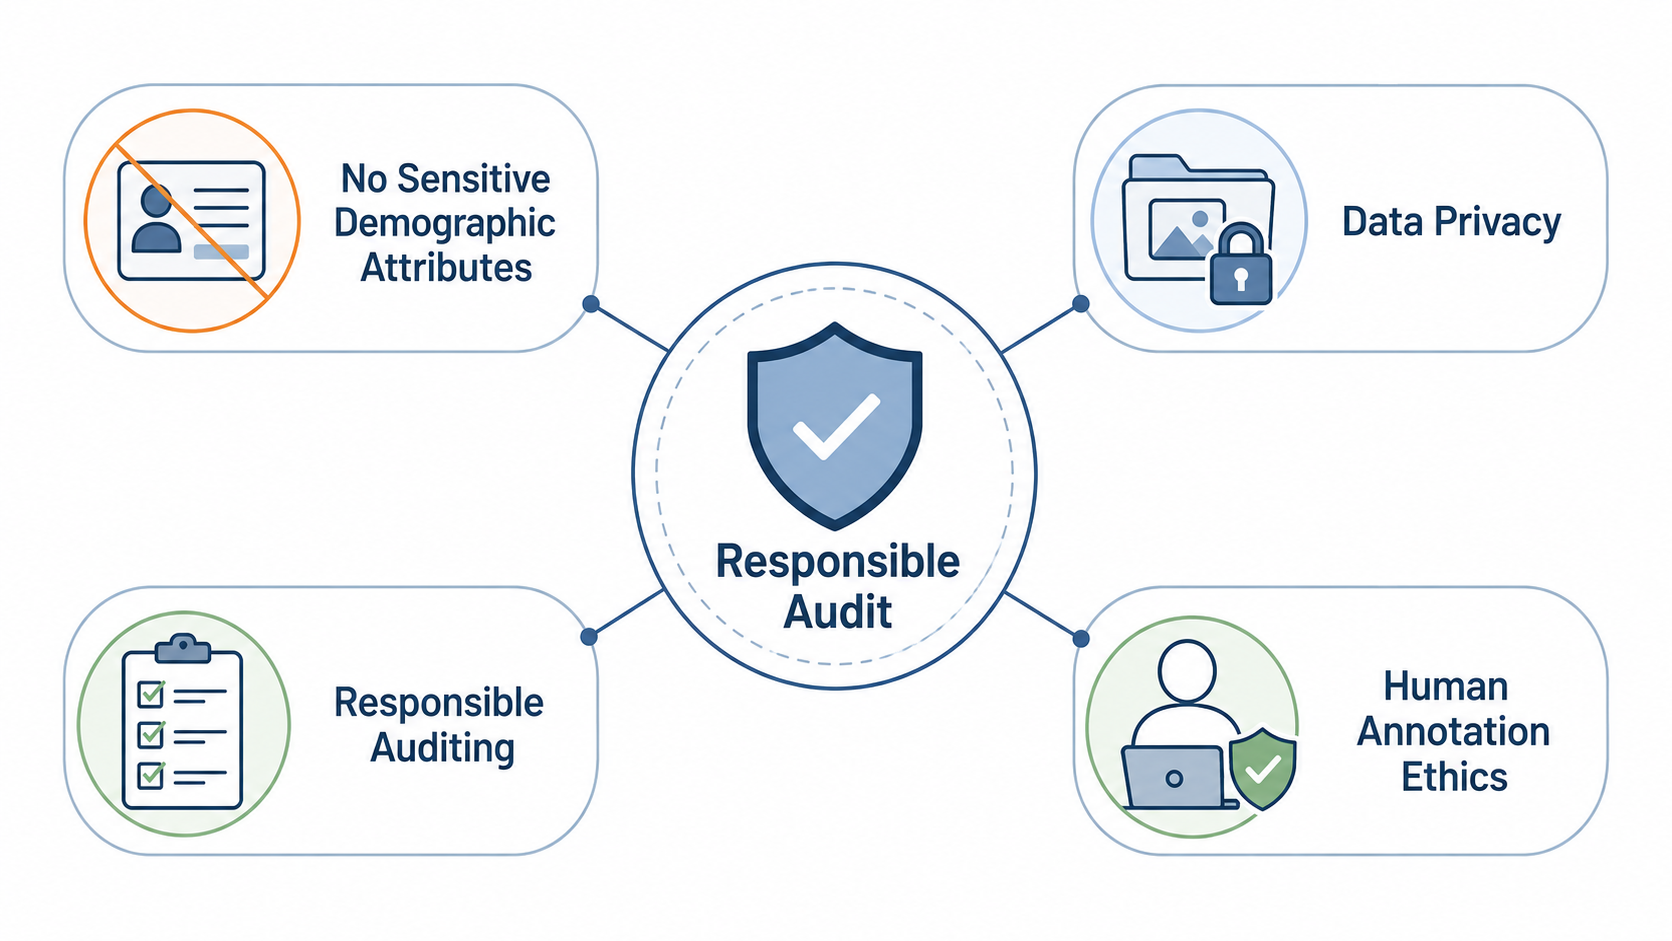
\includegraphics[width=0.95\linewidth]{figures/pictures/ethical_guardrails.png}
    \caption{Ethical Guardrails}
    \label{fig:ethical_guardrails}
\end{figure}

\section{Data Privacy}

The project relies on screenshots and interaction records, and these materials may contain sensitive information even when the accounts are newly created or controlled. For example, screenshots may accidentally capture account names, phone numbers, addresses, location information, payment interfaces, order details, recommendation histories, or other personal identifiers. Because the purpose of the study is to evaluate interface design features rather than personal information, such data should be blurred, removed, cropped, or excluded before analysis and presentation.

The dataset should retain only the information necessary for identifying and annotating dark pattern mechanisms. For instance, a screenshot showing a forced registration prompt, an obstructive cancellation path, or a pressure message may be useful for DPS annotation. However, the same screenshot should not preserve unrelated user identifiers or transaction details. This distinction is important because dark pattern auditing concerns the structure and behavior of the interface, not the private identity of the account holder.

Data minimization should therefore guide the entire workflow. Raw screenshots should be stored only when necessary, access should be limited to project members, and any public report figures should be carefully sanitized. If a report figure presents an example of interface interference or forced action, it should display only the relevant interface region. Similarly, annotation examples should describe interface mechanisms without including personal account information. These practices are consistent with the broader privacy principle that research data should be limited to what is necessary for the stated measurement objective.

\section{Responsible Auditing}

The goal of this project is not to attack, exploit, bypass, or disrupt mobile applications. The framework is designed to evaluate user-facing exposure to potentially manipulative interface practices under controlled profiles. This distinction is ethically important. The audit treats applications as black-box systems and records observable interface outcomes during ordinary interaction trajectories, following the general logic of external platform audits \cite{sandvig2014auditing,hannak2013personalization}. It does not attempt to access internal databases, reverse engineer private systems, overload services, circumvent authentication, or manipulate other users.

Responsible auditing also requires that the interaction procedure remain within normal user interaction boundaries. The profiles perform actions such as searching, browsing, scrolling, opening decision-related pages, closing pop-ups, or returning to previous screens. These actions resemble ordinary user behavior and are used only to observe whether dark pattern exposure differs across controlled profiles. The framework therefore measures what the application chooses to display in response to normal interactions, rather than forcing the application into abnormal states.

This ethical boundary also affects how findings should be interpreted. The project can report that certain profiles are associated with stronger exposure to interface interference or pressure-related mechanisms, or that some app categories show consistently high forced-action exposure. However, it should avoid overstating causality or claiming intentional discrimination without additional evidence. The appropriate interpretation is that the observed interface exposure patterns suggest profile-dependent differences that merit further investigation and accountability-oriented discussion.

\section{Human Annotation Ethics}

Human annotation is necessary because the DPS vector captures interface mechanisms that may require contextual judgment. However, annotation work should be designed to protect annotators as well as the privacy of the data subjects represented in screenshots. Annotators should not be exposed to unnecessary personal information. Before annotation, screenshots should be sanitized where possible, and annotation instructions should direct attention to visible interface mechanisms rather than user identity, account history, or personal content.

The annotation guidelines should define each DPS dimension in terms of observable evidence. For example, Interface Interference should be judged based on visual prominence, layout manipulation, or unequal presentation of options; Friction should be judged based on additional steps required to reject, cancel, or exit; Pressure should be judged based on countdowns, urgency messages, scarcity cues, or emotional persuasion; and Forced Action should be judged based on whether the interface requires an unrelated action before the user can proceed. This mechanism-focused approach helps reduce subjective moral judgment and keeps the annotation task aligned with prior dark pattern taxonomies \cite{gray2018darkpatterns,mathur2019darkpatterns,mathur2021whatmakesdark}.

Ambiguous cases should be discussed based on visible interface evidence rather than annotator assumptions. If a screenshot does not provide enough context to determine whether a design is deceptive, coercive, or merely inconvenient, the annotation should reflect that uncertainty through conservative labeling or discussion among annotators. This is especially important because dark pattern labels can carry normative implications. A responsible annotation process should therefore prioritize consistency, transparency, and evidence-based reasoning. In this sense, the DPS annotation framework is not only a technical measurement instrument, but also an ethical procedure for making claims about manipulative interface exposure in a careful and accountable manner.
